% StructRender conference paper draft (IEEEtran). Generated by docs/paper/build/build_paper.js from content.js.
% Compile with pdfLaTeX (Overleaf default). Placeholders marked [DETAILS REQUIRED] must be filled in.
\documentclass[conference]{IEEEtran}
\IEEEoverridecommandlockouts
\usepackage[T1]{fontenc}
\usepackage{cite}
\usepackage{amsmath,amssymb}
\usepackage{graphicx}
\usepackage{booktabs,tabularx,array}
\usepackage{textcomp}
\usepackage{url}
\DeclareUnicodeCharacter{00D7}{\ensuremath{\times}}
\DeclareUnicodeCharacter{221E}{\ensuremath{\infty}}
\DeclareUnicodeCharacter{2265}{\ensuremath{\geq}}
\DeclareUnicodeCharacter{2264}{\ensuremath{\leq}}
\DeclareUnicodeCharacter{1D4B2}{\ensuremath{\mathcal{W}}}
\DeclareUnicodeCharacter{00B7}{\ensuremath{\cdot}}
\DeclareUnicodeCharacter{2212}{\ensuremath{-}}
\DeclareUnicodeCharacter{03BA}{\ensuremath{\kappa}}
\DeclareUnicodeCharacter{00B0}{\ensuremath{^\circ}}
\DeclareUnicodeCharacter{2208}{\ensuremath{\in}}
\DeclareUnicodeCharacter{03BB}{\ensuremath{\lambda}}
\DeclareUnicodeCharacter{2207}{\ensuremath{\nabla}}
\DeclareUnicodeCharacter{03C1}{\ensuremath{\rho}}
\DeclareUnicodeCharacter{221A}{\ensuremath{\surd}}
\DeclareUnicodeCharacter{03C3}{\ensuremath{\sigma}}
\DeclareUnicodeCharacter{0394}{\ensuremath{\Delta}}
\begin{document}
\title{StructRender: Engine-Grounded Real-Time Neural Rendering of a Playable Game in Learned Painterly Styles}
\author{\IEEEauthorblockN{Kabilash S}
\IEEEauthorblockA{Dept. of Artificial Intelligence\\\relax
and Data Analytics\\\relax
Sri Ramachandra Faculty of\\\relax
Engineering and Technology\\\relax
SRIHER, Chennai, India\\\relax
kabilash0108@gmail.com}
\and
\IEEEauthorblockN{Pavitra P}
\IEEEauthorblockA{Dept. of Artificial Intelligence\\\relax
and Data Analytics\\\relax
Sri Ramachandra Faculty of\\\relax
Engineering and Technology\\\relax
SRIHER, Chennai, India\\\relax
fspavitra11@gmail.com}
\and
\IEEEauthorblockN{Dr. Vanitha V}
\IEEEauthorblockA{Dept. of Artificial Intelligence\\\relax
and Machine Learning\\\relax
Sri Ramachandra Faculty of\\\relax
Engineering and Technology\\\relax
SRIHER, Chennai, India}}
\maketitle
\begin{abstract}
Generative world models can synthesise game footage directly from pixels, but they hold no authoritative game state, so geometry, items and object identity can drift. We present StructRender, a renderer in which a deterministic game engine (Godot 4) keeps sole authority over physics, game logic and entity identity, and a neural network decides only how each frame looks. Every frame, the engine exports depth, normals, albedo, analytic motion vectors and an entity-identity map; a compact U-Net renders this structure in a painted style, fusing one frame of history warped by the engine's own motion and gated by an engine-derived disocclusion mask. A 16-dimensional style vector applied through FiLM lets one 8.4 M-parameter model render two styles and switch between them during play. Because no paired data exists for painted game frames, an offline Stable Diffusion 1.5 + depth-ControlNet teacher generates targets that must pass four pre-registered alignment gates. On held-out play sessions the model reaches 35.33 dB PSNR (oil) and 34.79 dB (watercolour) with sharpness ratios of 0.946 and 0.937, and flickers about half as much as its own teacher. Deployed through ONNX, TensorRT FP16 and a C++ GDExtension, it runs in the playable game at 44.6 fps on a laptop GPU (4.53 ms per network step), with no fallbacks over 3,000 frames, and the live frame matches the evaluated model to within one colour level. We also report two negative results: a window-transformer renderer never matched the U-Net at parameter parity, and a persistent per-entity appearance memory did not improve output on this data.
\end{abstract}
\begin{IEEEkeywords}
neural rendering, game engines, image-to-image translation, style transfer, diffusion models, temporal consistency, real-time inference
\end{IEEEkeywords}

\section{Introduction}\label{sec:intro}

Changing the \textit{look} of a game, for example rendering it as an oil painting, normally means re-authoring its materials and shaders. Neural rendering offers another route: a network learns to map scene information to an image with a target appearance \cite{neurend}. Game engines already compute that information every frame as per-pixel depth, normals and albedo, the G-buffer \cite{gbuffer}. A second line of work replaces the engine altogether: GameGAN, GameNGen and Genie learn to predict the next frame of a game from earlier frames and player actions \cite{gamegan,gamengen,genie}. Because such models hold no authoritative state, world facts such as a collected coin or the position of a wall can drift.
\begin{figure*}[!t]
\centering
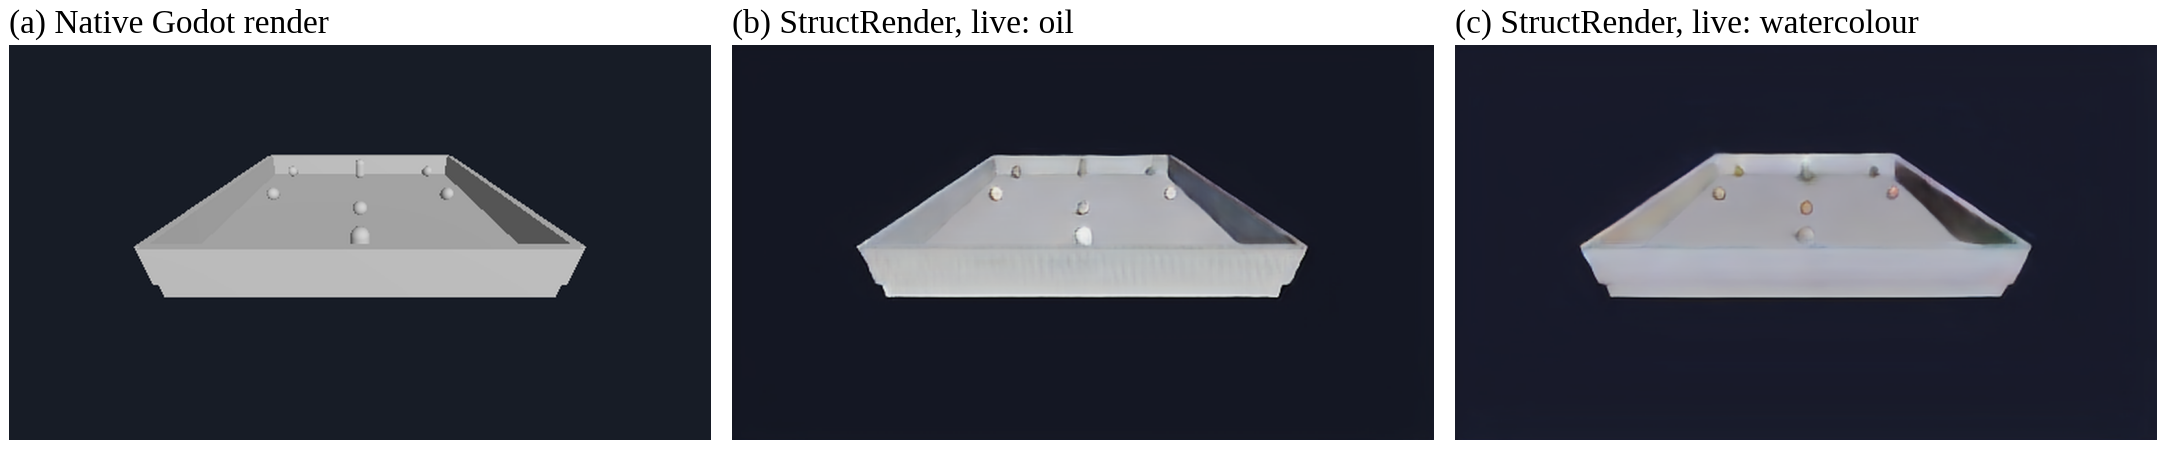
\includegraphics[width=1\textwidth]{figures/teaser.png}
\caption{One live frame of the playable game. (a) Godot's native render; (b), (c) the same frame rendered live by StructRender in its two learned styles. Physics, objects and positions come from the engine; only the appearance changes, and the style can be switched during play.}\label{fig:teaser}
\end{figure*}

StructRender takes the opposite position: \textbf{the engine is the single source of truth, and the network decides appearance only.} Every frame, the Godot engine \cite{godot} exports its structural buffers, and a compact convolutional network \cite{unet} renders them in a painted style (Fig.~\ref{fig:teaser}). Paired data for painterly game frames does not exist, so Stable Diffusion 1.5 \cite{ldm} with a depth ControlNet \cite{controlnet} is used offline only, to generate training targets. The network runs live through ONNX \cite{onnx}, TensorRT \cite{tensorrt} and C++, and because it never touches game state, a renderer error cannot become a gameplay error.

Three problems make this harder than per-frame style transfer. A diffusion teacher can invent geometry and is itself temporally unstable; per-frame stylisation flickers on video \cite{lai}; and the live renderer must fit an 8 GB laptop GPU while provably being the model that was evaluated. Our contributions are:
\begin{itemize}
\item \textbf{An engine-grounded design} in which structure is the input, engine motion drives temporal warping, and entity identity is used only as an address (masks and memory keys), never as a network input.
\item \textbf{Gated supervision from an offline diffusion teacher}, with four alignment gates fixed before the data existed, including a stylisation gate that rejects a teacher that changes nothing.
\item \textbf{StyleTemporalUNet}, a U-Net with a style-free encoder, engine-warped bottleneck history and a FiLM-modulated decoder, so one 8.39 M-parameter model renders two styles and keeps its history across a live style switch.
\item \textbf{A verified real-time deployment} at 44.6 fps with a link-by-link equivalence check between the evaluated and the live frame, and a pre-registered evaluation that reports two negative results: a window-transformer renderer and a persistent per-entity appearance memory.
\end{itemize}

\section{Related Work}\label{sec:related}

\textbf{Learned rendering from engine buffers.} Deep Shading \cite{deepshading} showed that a CNN can map G-buffer attributes to screen-space shading at interactive rates. Neural supersampling \cite{xiao} warps earlier frames with engine motion vectors and depth to reconstruct high-resolution images in real time. Enhancing Photorealism Enhancement \cite{epe} conditions an enhancement network on GTA V's G-buffers and trains it adversarially against real photographs. These works establish that engine buffers make neural rendering stable; none targets learned artistic styles, for which no real-image domain exists.

\textbf{Structure-to-image and video translation.} pix2pix \cite{pix2pix} translates label maps to images with a conditional GAN and a U-Net generator, but needs paired data. vid2vid \cite{vid2vid} adds flow-based warping for coherent video, and World-Consistent vid2vid \cite{wcvid2vid} keeps appearance consistent on revisits by projecting earlier output through a reconstructed point cloud, the closest analogue of our appearance-memory experiment. Both rely on estimated flow or geometry and heavy generators.

\textbf{Style, conditioning and diffusion.} Gatys et al.\ represented style by correlations of deep features \cite{gatys}; conditional instance normalisation stores many styles in one network \cite{cin}, and FiLM generalises this to a learned per-channel scale and shift \cite{film}, which our decoder uses. Diffusion models generate images by iterative denoising \cite{ddpm}, latent diffusion made them practical on consumer GPUs \cite{ldm}, partial noising trades faithfulness against change \cite{sdedit}, and ControlNet adds spatial conditioning through zero-initialised layers \cite{controlnet}, an idea we reuse so that every new mechanism starts as an exact no-op.

\textbf{Temporal consistency and generative games.} Lai et al.\ \cite{lai} remove flicker from per-frame processed video with temporal losses on optical-flow-warped frames; our temporal term follows the same principle with exact engine motion and an engine-derived disocclusion mask. GameGAN \cite{gamegan}, GameNGen \cite{gamengen} and Genie \cite{genie} learn playable simulators but keep game state implicit in pixels or latents, which motivates our engine-authoritative design.

\section{Method}\label{sec:method}

\subsection{System Overview}

Fig.~\ref{fig:arch} shows the system: an offline part that produces a validated dataset and a trained model, and a runtime loop that runs once per game frame inside Godot. The game is an arena collector (a player collecting coins while spawned enemies chase it) running Godot physics at 60 Hz. Override-shader passes re-render each frame as depth, normals, albedo and an entity-ID map; motion vectors are computed analytically from camera and entity transforms. A scripted recorder drives the game through its own input actions and advances exactly one physics step per frame with the scene paused while the passes render, so every buffer shows the same instant; a validator rejects sessions with schema, channel or sequence errors.
\begin{figure*}[!t]
\centering
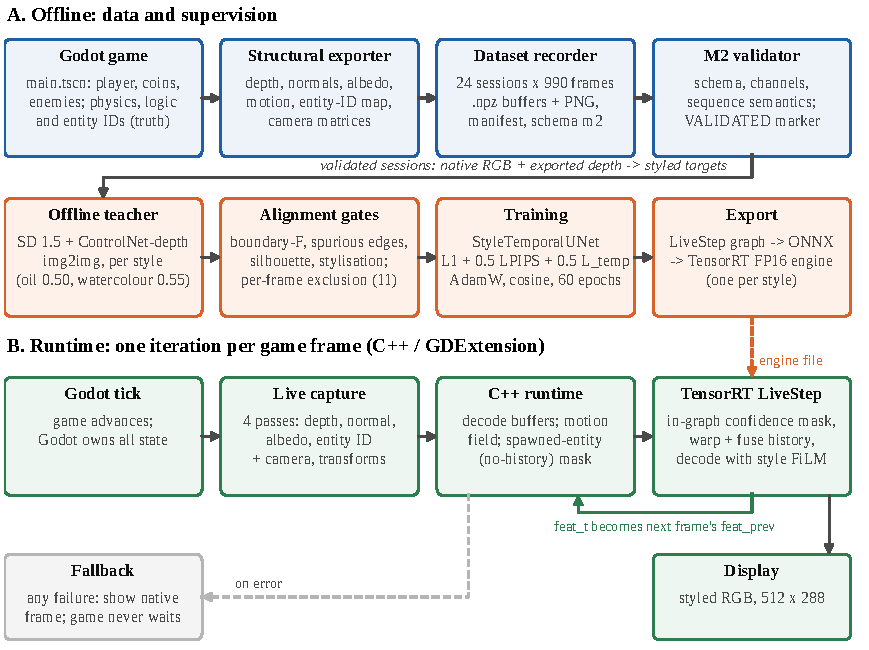
\includegraphics[width=0.82\textwidth]{figures/architecture.pdf}
\caption{System architecture. Offline (top): recording, gated teacher targets, training and export. Runtime (bottom): every game frame, Godot captures four passes, the C++ GDExtension computes motion and the mask of newly spawned entities and runs the TensorRT engine with the previous frame's features; any failure shows the native frame.}\label{fig:arch}
\end{figure*}

\textbf{Input encoding.} The network input has 7 channels: inverse depth, normals (3) and albedo (3), at 512 × 288. Depth \textit{d} in metres is bounded, with background (\textit{d} = ∞) mapped to 0:
\begin{equation}\label{eq:depth}
x_{\mathrm{depth}} = \frac{1}{1+d}.
\end{equation}

Motion and entity IDs are deliberately \textbf{not} input channels: motion is used for warping, and IDs are addresses, since a numeric ID channel would make a recycled ID look like the entity it replaced. No augmentation is used, because it would break the exact correspondence between structure, motion and target.

\subsection{Gated Diffusion Teacher}

For each validated frame and style, SD 1.5 \cite{sd15} img2img with a depth ControlNet \cite{cndepth}, conditioned on the engine's own depth, generates the target (24 steps, guidance 7.5, ControlNet scale 1.6; strength 0.50 for \textit{oil impasto} and 0.55 for a \textit{bold watercolour}; fixed seeds). Each target is scored against the engine's structure by the four gates of Table~\ref{tab:gates}, whose thresholds were fixed before the game data existed. Gate 4 exists because gates 1–3 are passed trivially by a teacher that changes nothing. Style strength was chosen by a pre-registered rule: the strongest setting with zero failures on a 45-frame probe, then on a full 990-frame session. A frame failing any gate in either style is excluded from both, together with every temporal sample that touches it; this removed 11 of 23,760 frames.
\begin{table}[!t]
\caption{Alignment gates (thresholds fixed before the data)}\label{tab:gates}
\centering
\footnotesize
\setlength{\tabcolsep}{4pt}
\begin{tabularx}{\columnwidth}{lXc}
\toprule
Gate & Measures & Pass \\
\midrule
1. Boundary F & structural edges preserved (2 px tolerance) & ≥ 0.60 \\
2. Spurious edges & strong edges with no structural support & ≤ 0.35 \\
3. Silhouettes & each entity of ≥ 200 px keeps its outline & ≥ 0.60 \\
4. Stylisation & colour-histogram L1 distance from the native frame & ≥ 0.15 \\
\bottomrule
\end{tabularx}
\end{table}

\subsection{Engine-Derived Confidence Mask}

A training sample is three consecutive frames. A per-pixel mask \textit{M}\textsubscript{t} decides which pixels may trust history. With 𝒲(·, \textit{V}\textsubscript{t}) the backward warp by the engine motion field \textit{V}\textsubscript{t}, and \textit{D} and \textit{N} depth and normals, the depth and normal disagreements \textit{e}\textsubscript{D} = |\textit{D}\textsubscript{t} − 𝒲(\textit{D}\textsubscript{t−1}, \textit{V}\textsubscript{t})| and \textit{e}\textsubscript{N} = 1 − \textit{N}\textsubscript{t} · 𝒲(\textit{N}\textsubscript{t−1}, \textit{V}\textsubscript{t}) give
\begin{equation}\label{eq:mask}
M_t = \exp\!\left(-\kappa_D\, e_D - \kappa_N\, e_N\right) H_t,
\end{equation}

with κ\textsubscript{D} = ln 2 / 0.175 m and κ\textsubscript{N} = ln 2 / (1 − cos 30°), so a depth step of 0.175 m or a normal change of 30° halves the confidence. \textit{H}\textsubscript{t} ∈ \{0, 1\} zeroes pixels with no valid history: the first frame, off-screen motion, background and newly spawned entities, found from the entity-ID map. The 0.175 m scale is the best separation (Youden index) between depth steps within surfaces and across silhouettes in the data. Fig.~\ref{fig:inputs} shows these quantities for a sealed test frame.
\begin{figure*}[!t]
\centering
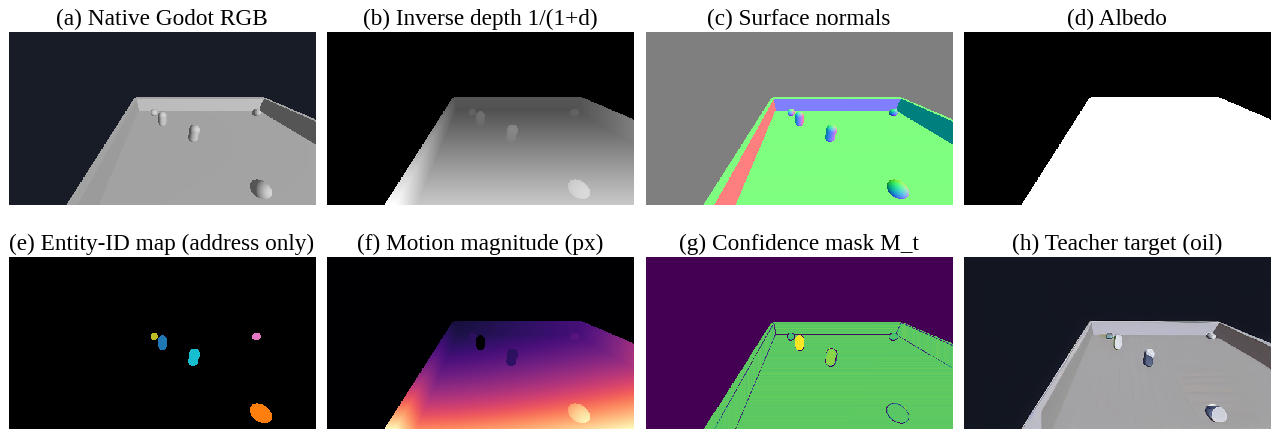
\includegraphics[width=1\textwidth]{figures/inputs.png}
\caption{One sealed test frame: (a) native render; (b)–(d) the seven input channels; (e) the entity-ID map, used only as an address; (f) engine motion magnitude; (g) the confidence mask \textit{M}\textsubscript{t}, low where history cannot be trusted (background, silhouettes, disocclusions); (h) the oil teacher target.}\label{fig:inputs}
\end{figure*}

\subsection{StyleTemporalUNet}

The deployed network (Fig.~\ref{fig:network}) has 8,394,915 parameters. \textbf{Encoder:} four levels, each two 3 × 3 convolutions with group normalisation (8 groups) \cite{groupnorm} and ReLU followed by 2 × 2 max pooling, give 32, 64, 128 and 256 channels; a bottleneck produces 512 channels at 18 × 32. The encoder reads only structure, never the style, so its features serve as history across a live style switch. \textbf{Temporal fusion:} the previous frame's bottleneck features \textit{F}\textsubscript{t−1} are warped by the engine motion, masked, and fused through a zero-initialised 1 × 1 convolution, so an untrained model equals the single-frame U-Net and history is ignored wherever \textit{M}\textsubscript{t} = 0:
\begin{equation}\label{eq:fusion}
F'_t = F_t + M_t \odot \mathrm{Conv}_{1\times1}\big(\big[F_t,\; M_t \odot \mathcal{W}(F_{t-1}, V_t)\big]\big).
\end{equation}

\textbf{Decoder:} each level upsamples by 2, concatenates the encoder skip and applies two convolution blocks modulated by FiLM \cite{film} from the selected style's learned 16-dimensional vector \textit{s}:
\begin{equation}\label{eq:film}
h' = h \odot (1 + \gamma_s) + \beta_s, \qquad [\gamma_s; \beta_s] = A_l\, s + b_l .
\end{equation}

Zero-initialised projections make an untrained two-style model exactly the single-style one. A 1 × 1 convolution and a sigmoid output RGB in [0, 1].
\begin{figure*}[!t]
\centering
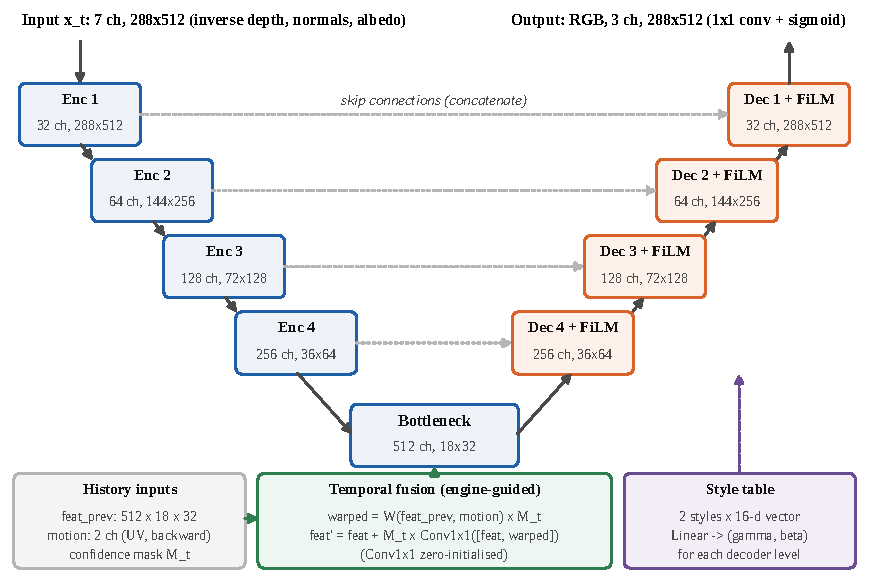
\includegraphics[width=0.8\textwidth]{figures/network.pdf}
\caption{StyleTemporalUNet: a style-free encoder, engine-warped temporal fusion at the bottleneck, and a decoder modulated by a 16-dimensional style vector through FiLM.}\label{fig:network}
\end{figure*}

\subsection{Training Objective}

With teacher target \textit{I}\textsubscript{t}, prediction \textit{Î}\textsubscript{t} and pixel \textit{p}, every model in this work is trained with
\begin{equation}\label{eq:loss}
\begin{aligned}\mathcal{L} = {}& \lVert \hat I_t - I_t \rVert_1 + 0.5\,\mathrm{LPIPS}(\hat I_t, I_t) \\ &+ 0.5\,\frac{\sum_p M_t\, |\hat I_t - \mathcal{W}(\hat I_{t-1}, V_t)|}{\sum_p M_t},\end{aligned}
\end{equation}

where LPIPS uses AlexNet features \cite{lpips}. The temporal term compares the prediction with its own warped predecessor under the same mask that the evaluation uses.

\subsection{Comparison Renderers and Appearance Memory}

For the ablation, Model A is the same U-Net without history and B adds the temporal fusion. \textit{StructFormer} (C) replaces the U-Net with a convolutional stem, a window-attention encoder and decoder \cite{swin} and a convolutional head; D adds the temporal fusion, E adds entity-masked cross-attention, and the control N feeds the raw entity ID as an input channel instead. \textbf{EPAM} (Engine-Keyed Persistent Appearance Memory) extends E with a session-local memory keyed by the engine's entity key: an entity's descriptor is blended into its slot by an exponential moving average with decay λ = 0.9 when the entity is visible enough, frozen while it is out of view, deleted when it is destroyed and cleared on a style change. Setting λ = 0 reduces EPAM to the current descriptor, so Model F (λ = 0.9) and its control F0 (λ = 0) train through identical code, data, schedule and selection rule, and F − F0 measures the memory alone. All rungs were trained at parameter parity (0.9–1.1×).

\subsection{Runtime}

One step of the network including the confidence mask (\textit{LiveStep}) is exported to ONNX and compiled to one TensorRT FP16 engine per style on the target laptop. Each game frame, Godot captures the four passes; a C++ GDExtension \cite{godotcpp} computes motion and the no-history mask of newly spawned entities, runs the engine with the previous frame's features, displays the result and keeps the new features. Any failure shows the native frame, so the game never waits for the renderer.

\section{Experimental Setup}\label{sec:setup}

Both datasets were recorded by the project with the same exporter, recorder and validator (Table~\ref{tab:data}). The \textbf{game dataset}, recorded from the playable game, trained and tested the deployed model. The \textbf{seed-scene dataset}, recorded earlier from an arena built in code, was used for the ablation ladder. Splits are by whole session and were fixed before any target or model existed; the test splits were scored once, at the end. All recording, generation, training and deployment ran on one laptop with an AMD Ryzen 9 8940HX CPU and an NVIDIA RTX 5060 Laptop GPU (8 GB), using PyTorch \cite{pytorch} and TensorRT 11.
\begin{table}[!t]
\caption{Data and training configuration}\label{tab:data}
\centering
\footnotesize
\setlength{\tabcolsep}{4pt}
\begin{tabularx}{\columnwidth}{lX}
\toprule
Item & Setting \\
\midrule
Game dataset & 24 sessions × 990 frames (23,760) at 512 × 288; split 18 / 3 / 3 sessions (17,820 / 2,970 / 2,970 frames); 11 frames excluded by the gates \\
Seed-scene dataset & 29 valid sessions (28,710 frames); split 21 / 4 / 4 (20,790 / 3,960 / 3,960) \\
Training samples & 35,526 (both styles); 5,936 validation frames \\
Optimiser & AdamW \cite{adamw}, learning rate 2 × 10\textsuperscript{−4}, weight decay 10\textsuperscript{−4}, cosine schedule \cite{sgdr} \\
Batch, precision & 4 × gradient accumulation 2; bfloat16 \\
Epochs, selection & 60, validation every 2; lowest validation L1; seed 20260905 \\
Wall time & 29.2 h; best epoch 49 (validation L1 0.007435) \\
\bottomrule
\end{tabularx}
\end{table}

\textbf{Metrics.} We report PSNR, SSIM \cite{ssim} and LPIPS \cite{lpips}. Because pixel-error regressors blur when targets are uncertain \cite{pd}, every result is paired with a \textbf{sharpness ratio}, the high-pass energy of the prediction relative to the target, with Sobel gradients ∇ of luma \textit{Y} summed over the test set; a ratio of 0.90 corresponds to roughly a 1-pixel Gaussian blur of the target, and 0.90 is the gate:
\begin{equation}\label{eq:sharp}
S = \frac{\sum \lVert \nabla Y(\hat I) \rVert^2}{\sum \lVert \nabla Y(I) \rVert^2}.
\end{equation}

To show that the style is learned rather than ignored, the \textbf{travel ratio} ρ compares how far the model and the teacher move the 32-bin colour histogram \textit{h} away from the native frame \textit{I}\textsubscript{nat} (gate ≥ 0.80):
\begin{equation}\label{eq:travel}
\rho = \frac{\lVert h(\hat I) - h(I_{\mathrm{nat}}) \rVert_1}{\lVert h(I) - h(I_{\mathrm{nat}}) \rVert_1}.
\end{equation}

\textbf{Temporal error} (flicker) is the mean difference between a frame and its warped predecessor on confident pixels, over pairs with at least 1 pixel of median motion; since a frozen output scores zero, it is always read together with sharpness:
\begin{equation}\label{eq:te}
\mathrm{TE} = \frac{\sum_p M_t\, |I_t - \mathcal{W}(I_{t-1}, V_t)|}{\sum_p M_t}.
\end{equation}

\textbf{Noise threshold.} A difference between two single runs is claimed only if it exceeds 2√2 · \textit{sd}\textsubscript{rel}, where \textit{sd}\textsubscript{rel} is the relative seed-to-seed standard deviation measured with three seeds on the seed scene. Live frame rate is 1000 divided by the median loop time in milliseconds for the whole loop; network latency is the median of 500 standalone TensorRT runs.

\section{Results}\label{sec:results}

\subsection{Ablation Ladder}

Table~\ref{tab:ladder} and Fig.~\ref{fig:ladder} report every rung on the same 3,960 sealed test frames of the seed scene, scored by one evaluation script; temporal error uses 501 moving frame pairs.
\begin{table*}[!t]
\caption{Ablation ladder on the sealed seed-scene test split (3,960 frames)}\label{tab:ladder}
\centering
\footnotesize
\setlength{\tabcolsep}{4pt}
\begin{tabular}{lcccccc}
\toprule
Rung & PSNR (dB) & SSIM & LPIPS & Sharpness & Temporal error & Params \\
\midrule
A  U-Net & \textbf{34.04} & \textbf{0.9747} & \textbf{0.0459} & \textbf{0.912} & 0.003175 & 7.85 M \\
B  U-Net + temporal & 33.64 & 0.9734 & 0.0489 & 0.897 & \textbf{0.002692} (−15.2 \%) & 8.38 M \\
C  StructFormer & 33.86 & 0.9728 & 0.0466 & 0.853 & 0.004191 & 7.78 M \\
D  StructFormer + temporal & 33.56 & 0.9727 & 0.0485 & 0.858 & 0.003741 (−10.7 \%) & 8.24 M \\
E  StructFormer + entity & 33.79 & 0.9726 & 0.0463 & 0.884 & 0.004172 & 7.05 M \\
N  raw-ID control & 33.86 & 0.9732 & 0.0459 & 0.880 & – & 7.78 M \\
Teacher targets / native engine & – & – & – & – & 0.006265 / 0.000241 & – \\
\bottomrule
\end{tabular}
\end{table*}
\begin{figure}[!t]
\centering
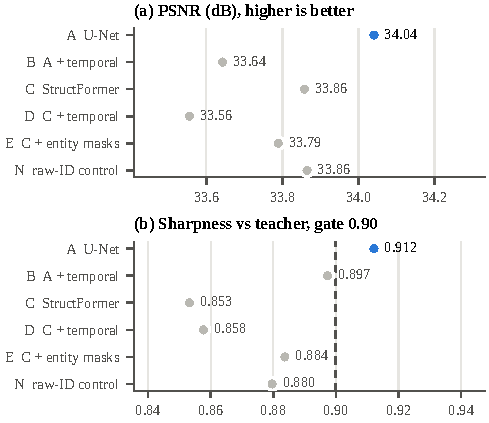
\includegraphics[width=\columnwidth]{figures/ladder.pdf}
\caption{Ablation ladder on the sealed seed-scene test split. The plain U-Net (A, blue) leads on PSNR and is the only rung above the 0.90 sharpness gate (dashed).}\label{fig:ladder}
\end{figure}

\textbf{The plain U-Net (A) is best on every image-quality metric} and is the only rung above the sharpness gate. StructFormer's sharpness was 0.833, 0.886 and 0.851 at 644, 10,890 and 20,790 training frames, against a pre-recorded projection of 0.898, so more data did not close the gap: at this scale the convolutional inductive bias suits the task better. \textbf{Temporal conditioning cuts flicker on both backbones}, by 15.2 \% (B vs.\ A) and 10.7 \% (D vs.\ C), well beyond the pre-registered threshold of 3.85 \% (2√2 × 1.36 \%), at a cost of 1.8–3.9 \% in per-frame L1. Because flicker is the more visible defect in play, the U-Net with temporal fusion was chosen for the game. \textbf{Entity awareness} sharpens StructFormer (+0.015 over C across three seeds, 2.5σ), but the raw-ID control N recovers about 87 \% of that gain: with two or three stable IDs in this scene, exposing the IDs is enough.

\subsection{The Deployed Two-Style Model}

The deployed model is rung B (U-Net with temporal fusion) trained on the game data with both styles. Table~\ref{tab:game} reports it on the game's three sealed test sessions, 2,968 frames per style, each evaluated with its real previous frame. Both styles clear the sharpness and travel gates and beat the do-nothing baseline (showing the native frame) by 7.3–7.8 dB. Sharing one model between two styles costs oil 0.10 dB against an oil-only model, which is not claimed as significant with one run per model. The style switch is real rather than a blend: on a sampled test session each style's output is about 4× closer to its own targets than to the other style's, reproducing 93 \% of the difference between the two teachers.
\begin{table}[!t]
\caption{Game test sessions (2,968 frames per style)}\label{tab:game}
\centering
\scriptsize
\setlength{\tabcolsep}{2.5pt}
\begin{tabular}{lcccccc}
\toprule
Model, style & PSNR & SSIM & LPIPS & Sharp. & ρ & TE / teach. \\
\midrule
Two-style, oil & 35.33 & 0.9807 & 0.0225 & 0.946 & 0.995 & 0.54× \\
Two-style, watercolour & 34.79 & 0.9786 & 0.0243 & 0.937 & 0.987 & 0.48× \\
Oil-only (reference) & 35.43 & 0.9814 & 0.0216 & 0.946 & 0.980 & 0.54× \\
Native frame, oil / w.c. & 28.06 / 26.96 & – & – & – & – & – \\
\bottomrule
\end{tabular}
\end{table}
\begin{figure*}[!t]
\centering
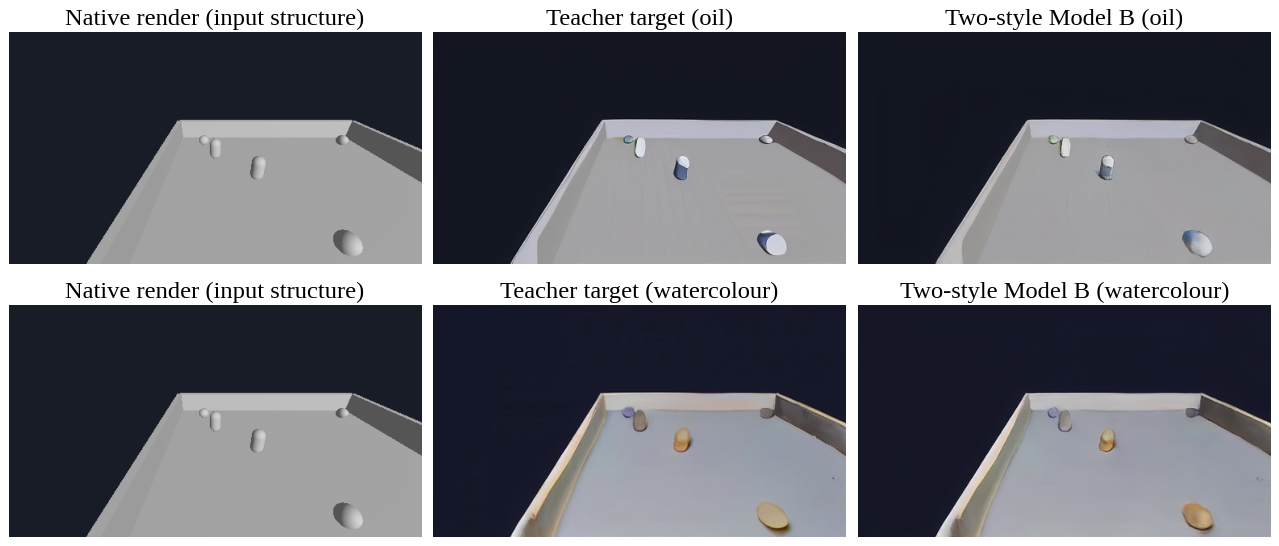
\includegraphics[width=0.9\textwidth]{figures/qualitative.png}
\caption{A sealed test frame rendered through exactly the evaluated path: native input, teacher target and model output for both styles. Geometry is the engine's in every column; only appearance changes.}\label{fig:qual}
\end{figure*}

Fig.~\ref{fig:qual} shows a sealed test frame. The styles are mild because the game is grey and plainly lit, and stronger settings fail the gates. Fig.~\ref{fig:training} shows the training run: validation L1 reaches its minimum of 0.007435 at epoch 49 and then flattens, while the temporal term \textit{rises} as the initially smooth, and therefore stable, output acquires the teacher's texture. This is why temporal error is never reported without sharpness.
\begin{figure}[!t]
\centering
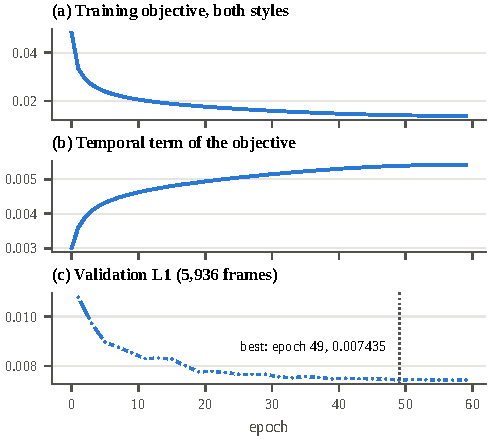
\includegraphics[width=\columnwidth]{figures/training.pdf}
\caption{Training of the deployed model: (a) full objective, (b) its temporal term, which grows as the output acquires texture, and (c) validation L1 on 5,936 frames.}\label{fig:training}
\end{figure}

\subsection{Temporal Stability}

The renderer flickers about half as much as its own teacher (0.54× for oil, 0.48× for watercolour; Fig.~\ref{fig:flicker}), measured on 2,451 moving frame pairs, but still about 57× the native engine, which bounds what a per-frame teacher can supervise. History also matters for image quality: run as a cold start every frame, the same model drops from 35.33 to 33.58 dB (oil) and from 34.79 to 32.82 dB (watercolour) (Fig.~\ref{fig:history}), so the live runtime feeds the previous frame's features back every frame.
\begin{figure}[!t]
\centering
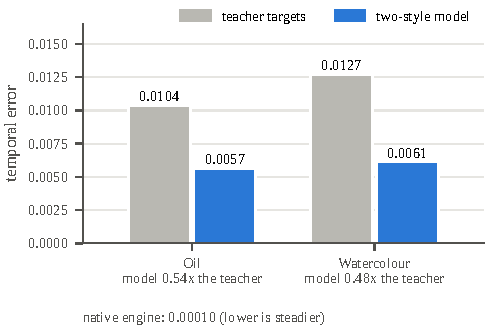
\includegraphics[width=\columnwidth]{figures/flicker.pdf}
\caption{Temporal error on the game's test sessions: the teacher's targets and the two-style model. Lower is steadier.}\label{fig:flicker}
\end{figure}
\begin{figure}[!t]
\centering
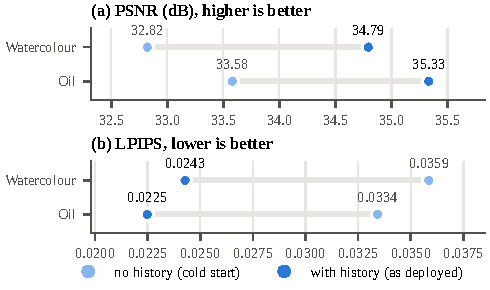
\includegraphics[width=\columnwidth]{figures/history.pdf}
\caption{The same model with and without its one frame of engine-warped history, on the same test frames.}\label{fig:history}
\end{figure}

\subsection{Live Deployment}

To ensure that the game shows the evaluated model, each link from evaluator to screen was checked with identical inputs (Table~\ref{tab:live}). The FP16 engine passed a tolerance fixed before measurement (mean |ΔPSNR| < 0.05 dB and mean pixel change < 1/255) with 0.044 / 0.039 dB and 0.0004; its few larger pixel differences lie on one-pixel object outlines. FP16 is 27 \% faster than strict FP32 (Fig.~\ref{fig:live}), so it ships. Live in the playable game the whole loop, including the four capture passes, motion, inference and display, runs at 44.6 fps (oil) and 44.7 fps (watercolour) against a 30 fps target, with no fallback over 3,000 frames; in a manual play session with desktop applications open, 2,059 styled frames ran at 40.1 and 38.0 fps, again with no fallback.
\begin{table}[!t]
\caption{Evaluator-to-screen equivalence and live criteria}\label{tab:live}
\centering
\footnotesize
\setlength{\tabcolsep}{4pt}
\begin{tabularx}{\columnwidth}{XX}
\toprule
Check & Result \\
\midrule
Exported LiveStep vs.\ Python evaluator (RGB) & max 2.4 × 10\textsuperscript{−6} \\
TensorRT strict FP32 vs.\ PyTorch (RGB / features) & 1.6 × 10\textsuperscript{−6} / 7.3 × 10\textsuperscript{−6} \\
C++ motion vs.\ engine motion (120 frames) & 7.5 × 10\textsuperscript{−8} (normalised UV) \\
Live frame vs.\ evaluated model & ≤ 1/255 (rounding); 0 pixels above \\
Spawned enemy: no-history pixels, C++ vs.\ engine & 998 = 998 pixels \\
Stability, 3,000 live frames & 0 fallbacks; median 22.4 vs.\ 22.3 ms (first vs.\ second half); p99 25.2 ms \\
Forced renderer failures & 8 of 8 fell back to the native frame; play continued \\
\bottomrule
\end{tabularx}
\end{table}
\begin{figure}[!t]
\centering
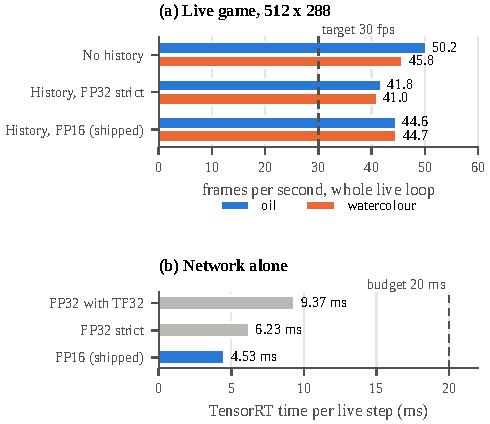
\includegraphics[width=\columnwidth]{figures/live.pdf}
\caption{(a) Frame rate of the whole live loop in the playable game, by configuration and style. (b) TensorRT time per network step alone; the shipped FP16 engine takes 4.53 ms.}\label{fig:live}
\end{figure}

\subsection{Persistent Appearance Memory: A Negative Result}

EPAM does not improve the output. On 3,912 sealed test clips, the sharpness of F (memory on) minus F0 (memory off) is −0.0127 (0.8829 vs.\ 0.8956), inside the pre-registered threshold of 0.0206 and in the wrong direction; the 1.03 \% lower L1 of F is also inside noise and not claimed. The memory's lifecycle rules (retrieval after leaving view, no leakage after destruction, clearing on a style change) are met and covered by 17 tests. Three further measurements agree that this data offers a memory nothing to recover: residual appearance correlation is at most 0.037 beyond 30 ticks, appearance does not decay with time unseen, and anchoring the teacher's noise to each entity does not create a persistent per-entity look. The most consistent reading is that the diffusion teacher re-invents each object's appearance every frame, so an average over frames only reinforces the blur; testing EPAM properly needs a temporally consistent teacher or authored per-entity textures.

\section{Limitations}\label{sec:limits}

The evidence covers one simple game and two mild styles; the game uses flat, untextured geometry, and stronger styles fail the alignment gates. Teacher flicker bounds the achievable temporal quality. The game models were trained once, so small differences between them are not claimed. Recording used scripted rather than human play, and the 11 excluded frames are the hardest views to align, which are therefore slightly under-represented. A move to 768 × 432 was stopped before the bulk run because the teacher's look changes with resolution: the best re-tuned settings were no closer to the committed look than the unstyled frame (LPIPS 0.094 / 0.100 vs.\ 0.099 / 0.117).

\section{Conclusion}\label{sec:conclusion}

StructRender adds a learned painterly style to a playable game without letting a neural network decide anything about the game. The engine's own structure, motion and identity drive a gated diffusion teacher and a temporally conditioned two-style U-Net, which runs live at 44.6 fps on a laptop GPU and provably shows the evaluated model. The pre-registered evaluation also reports where the more ambitious components did not help: a window transformer did not beat the U-Net, and per-entity appearance memory found nothing to recover in this data. Future work includes a temporally consistent teacher, a re-test of EPAM in scenes with many entities, occlusions and recycled IDs, higher resolution with a matched look, and evaluation on more games and on human play.

\begin{thebibliography}{34}
\bibitem{neurend} A. Tewari et al., ``State of the art on neural rendering,'' \textit{Comput. Graph. Forum}, vol. 39, no. 2, pp. 701–727, 2020, doi: 10.1111/cgf.14022.
\bibitem{gbuffer} T. Saito and T. Takahashi, ``Comprehensible rendering of 3-D shapes,'' \textit{ACM SIGGRAPH Comput. Graph.}, vol. 24, no. 4, pp. 197–206, 1990, doi: 10.1145/97880.97901.
\bibitem{gamegan} S. W. Kim, Y. Zhou, J. Philion, A. Torralba, and S. Fidler, ``Learning to simulate dynamic environments with GameGAN,'' in \textit{Proc. IEEE/CVF Conf. Comput. Vis. Pattern Recognit. (CVPR)}, 2020, pp. 1228–1237, doi: 10.1109/CVPR42600.2020.00131.
\bibitem{gamengen} D. Valevski, Y. Leviathan, M. Arar, and S. Fruchter, ``Diffusion models are real-time game engines,'' in \textit{Proc. Int. Conf. Learn. Represent. (ICLR)}, 2025, arXiv:2408.14837.
\bibitem{genie} J. Bruce et al., ``Genie: Generative interactive environments,'' arXiv preprint arXiv:2402.15391, 2024.
\bibitem{godot} Godot Engine contributors, ``Godot Engine documentation.'' [Online]. Available: \url{https://docs.godotengine.org/en/stable/} (accessed Oct. 23, 2026).
\bibitem{unet} O. Ronneberger, P. Fischer, and T. Brox, ``U-Net: Convolutional networks for biomedical image segmentation,'' in \textit{Medical Image Computing and Computer-Assisted Intervention – MICCAI 2015} (Lecture Notes in Computer Science). Cham, Switzerland: Springer, 2015, pp. 234–241, doi: 10.1007/978-3-319-24574-4\_28.
\bibitem{ldm} R. Rombach, A. Blattmann, D. Lorenz, P. Esser, and B. Ommer, ``High-resolution image synthesis with latent diffusion models,'' in \textit{Proc. IEEE/CVF Conf. Comput. Vis. Pattern Recognit. (CVPR)}, 2022, pp. 10674–10685, doi: 10.1109/CVPR52688.2022.01042.
\bibitem{controlnet} L. Zhang, A. Rao, and M. Agrawala, ``Adding conditional control to text-to-image diffusion models,'' in \textit{Proc. IEEE/CVF Int. Conf. Comput. Vis. (ICCV)}, 2023, pp. 3813–3824, doi: 10.1109/ICCV51070.2023.00355.
\bibitem{onnx} ONNX Project, ``Open Neural Network Exchange (ONNX).'' [Online]. Available: \url{https://onnx.ai/} (accessed Oct. 23, 2026).
\bibitem{tensorrt} NVIDIA Corporation, ``NVIDIA TensorRT documentation.'' [Online]. Available: \url{https://docs.nvidia.com/deeplearning/tensorrt/latest/} (accessed Oct. 23, 2026).
\bibitem{lai} W.-S. Lai, J.-B. Huang, O. Wang, E. Shechtman, E. Yumer, and M.-H. Yang, ``Learning blind video temporal consistency,'' in \textit{Computer Vision – ECCV 2018} (Lecture Notes in Computer Science). Cham, Switzerland: Springer, 2018, pp. 179–195, doi: 10.1007/978-3-030-01267-0\_11.
\bibitem{deepshading} O. Nalbach, E. Arabadzhiyska, D. Mehta, H.-P. Seidel, and T. Ritschel, ``Deep shading: Convolutional neural networks for screen space shading,'' \textit{Comput. Graph. Forum}, vol. 36, no. 4, pp. 65–78, 2017, doi: 10.1111/cgf.13225.
\bibitem{xiao} L. Xiao, S. Nouri, M. Chapman, A. Fix, D. Lanman, and A. Kaplanyan, ``Neural supersampling for real-time rendering,'' \textit{ACM Trans. Graph.}, vol. 39, no. 4, 2020, doi: 10.1145/3386569.3392376.
\bibitem{epe} S. R. Richter, H. A. Alhaija, and V. Koltun, ``Enhancing photorealism enhancement,'' \textit{IEEE Trans. Pattern Anal. Mach. Intell.}, vol. 45, no. 2, pp. 1700–1715, 2023, doi: 10.1109/TPAMI.2022.3166687.
\bibitem{pix2pix} P. Isola, J.-Y. Zhu, T. Zhou, and A. A. Efros, ``Image-to-image translation with conditional adversarial networks,'' in \textit{Proc. IEEE Conf. Comput. Vis. Pattern Recognit. (CVPR)}, 2017, pp. 5967–5976, doi: 10.1109/CVPR.2017.632.
\bibitem{vid2vid} T.-C. Wang, M.-Y. Liu, J.-Y. Zhu, G. Liu, A. Tao, J. Kautz, and B. Catanzaro, ``Video-to-video synthesis,'' in \textit{Advances in Neural Information Processing Systems (NeurIPS)}, 2018, arXiv:1808.06601.
\bibitem{wcvid2vid} A. Mallya, T.-C. Wang, K. Sapra, and M.-Y. Liu, ``World-consistent video-to-video synthesis,'' in \textit{Computer Vision – ECCV 2020} (Lecture Notes in Computer Science). Cham, Switzerland: Springer, 2020, pp. 359–378, doi: 10.1007/978-3-030-58598-3\_22.
\bibitem{gatys} L. A. Gatys, A. S. Ecker, and M. Bethge, ``Image style transfer using convolutional neural networks,'' in \textit{Proc. IEEE Conf. Comput. Vis. Pattern Recognit. (CVPR)}, 2016, pp. 2414–2423, doi: 10.1109/CVPR.2016.265.
\bibitem{cin} V. Dumoulin, J. Shlens, and M. Kudlur, ``A learned representation for artistic style,'' in \textit{Proc. Int. Conf. Learn. Represent. (ICLR)}, 2017, arXiv:1610.07629.
\bibitem{film} E. Perez, F. Strub, H. de Vries, V. Dumoulin, and A. Courville, ``FiLM: Visual reasoning with a general conditioning layer,'' in \textit{Proc. AAAI Conf. Artif. Intell.}, vol. 32, no. 1, 2018, doi: 10.1609/aaai.v32i1.11671.
\bibitem{ddpm} J. Ho, A. Jain, and P. Abbeel, ``Denoising diffusion probabilistic models,'' in \textit{Advances in Neural Information Processing Systems (NeurIPS)}, 2020, arXiv:2006.11239.
\bibitem{sdedit} C. Meng, Y. He, Y. Song, J. Song, J. Wu, J.-Y. Zhu, and S. Ermon, ``SDEdit: Guided image synthesis and editing with stochastic differential equations,'' in \textit{Proc. Int. Conf. Learn. Represent. (ICLR)}, 2022, arXiv:2108.01073.
\bibitem{sd15} Hugging Face model repository ``stable-diffusion-v1-5/stable-diffusion-v1-5,'' revision 451f4fe1. [Online]. Available: \url{https://huggingface.co/stable-diffusion-v1-5/stable-diffusion-v1-5} (accessed Oct. 23, 2026).
\bibitem{cndepth} Hugging Face model repository ``lllyasviel/sd-controlnet-depth,'' revision 35e42a3e. [Online]. Available: \url{https://huggingface.co/lllyasviel/sd-controlnet-depth} (accessed Oct. 23, 2026).
\bibitem{groupnorm} Y. Wu and K. He, ``Group normalization,'' in \textit{Computer Vision – ECCV 2018} (Lecture Notes in Computer Science). Cham, Switzerland: Springer, 2018, pp. 3–19, doi: 10.1007/978-3-030-01261-8\_1.
\bibitem{lpips} R. Zhang, P. Isola, A. A. Efros, E. Shechtman, and O. Wang, ``The unreasonable effectiveness of deep features as a perceptual metric,'' in \textit{Proc. IEEE/CVF Conf. Comput. Vis. Pattern Recognit. (CVPR)}, 2018, pp. 586–595, doi: 10.1109/CVPR.2018.00068.
\bibitem{swin} Z. Liu, Y. Lin, Y. Cao, H. Hu, Y. Wei, Z. Zhang, S. Lin, and B. Guo, ``Swin Transformer: Hierarchical vision transformer using shifted windows,'' in \textit{Proc. IEEE/CVF Int. Conf. Comput. Vis. (ICCV)}, 2021, pp. 9992–10002, doi: 10.1109/ICCV48922.2021.00986.
\bibitem{godotcpp} Godot Engine contributors, ``godot-cpp: C++ bindings for the Godot script API (GDExtension),'' GitHub repository. [Online]. Available: \url{https://github.com/godotengine/godot-cpp} (accessed Oct. 23, 2026).
\bibitem{pytorch} A. Paszke et al., ``PyTorch: An imperative style, high-performance deep learning library,'' in \textit{Advances in Neural Information Processing Systems (NeurIPS)}, 2019, arXiv:1912.01703.
\bibitem{adamw} I. Loshchilov and F. Hutter, ``Decoupled weight decay regularization,'' in \textit{Proc. Int. Conf. Learn. Represent. (ICLR)}, 2019, arXiv:1711.05101.
\bibitem{sgdr} I. Loshchilov and F. Hutter, ``SGDR: Stochastic gradient descent with warm restarts,'' in \textit{Proc. Int. Conf. Learn. Represent. (ICLR)}, 2017, arXiv:1608.03983.
\bibitem{ssim} Z. Wang, A. C. Bovik, H. R. Sheikh, and E. P. Simoncelli, ``Image quality assessment: From error visibility to structural similarity,'' \textit{IEEE Trans. Image Process.}, vol. 13, no. 4, pp. 600–612, 2004, doi: 10.1109/TIP.2003.819861.
\bibitem{pd} Y. Blau and T. Michaeli, ``The perception-distortion tradeoff,'' in \textit{Proc. IEEE/CVF Conf. Comput. Vis. Pattern Recognit. (CVPR)}, 2018, pp. 6228–6237, doi: 10.1109/CVPR.2018.00652.
\end{thebibliography}
\end{document}
